\documentclass[conference]{IEEEtran}
\usepackage{times}
\usepackage{graphicx}
\graphicspath{ {./images/} }

% numbers option provides compact numerical references in the text. 
\usepackage[numbers]{natbib}
\usepackage{multicol}
\usepackage[bookmarks=true]{hyperref}

\pdfinfo{
   /Author (DRAGNUTA Tiberiu Theodor)
   /Title  (Wireless Multimedia Sensor Networks)
   /CreationDate (D:20210909120000)
   /Subject (Sensors)
   /Keywords (network; sensor; multimedia; gateway; IP; wireless)
}

\begin{document}

% paper title
\title{Wireless Multimedia Sensor Networks

}

%paper author
\author{DRĂGNUȚĂ Tiberiu Theodor for Research and practice activity Semester 1}


\maketitle

\begin{abstract}
The internet of things (IoT) represents a vast number of devices, sensors, objects that are connected to the internet being able to share data between themselves. The internet-connected devices use built-in sensors and they are able to collect and transfer data over a network without human-to-human or human-to-computer interaction being needed.
\end{abstract}

\IEEEpeerreviewmaketitle

\section{Introduction}
A wireless sensor network (WSN) is made of wirelessly interconnected devices which have the ability to interact with each other and with their surrounded environment by controlling and sensing physical parameters.  The sensor sends such collected data (called as scalar data), usually via radio transmitter, to a command center (sink) either directly or through multiple wireless hops (from \citet{Hamd01})
Wireless Multimedia Sensor Networks (WMSNs) are self-organizing systems of embedded devices deployed to retrieve, distributively process in real-time, store, correlate, and fuse multimedia streams originated from heterogeneous sources.
\\ \indent Some of the applications of these networks are the following: Multimedia Surveillance Sensor Networks, Traffic Avoidance, Enforcement, and Control Systems, Industrial Process Control, Environmental and Structural Monitoring, Advanced Health Care Delivery, Storage of potentially relevant activities and many more. (from \citet{Inaf02}
\\ \indent Wireless Sensor Networks have been the focused by many researchers during the last decade, all due to the advances in low power and low cost hardware. As mentioned, this continuously growing focus in WSNs and WMSNs can be used to support and develop new applications such as intelligent homes, health applications, environment control, etc. An advantage of the WMSNs over the WSN is the usage of the cheap CMOS cameras and microphones which are verry effective and can provide rich media content. (from \citet{Hamd01})


\section{Wireless Multimedia Network Sensors}

Most of the wireless sensor networks require networking and programming skills, for example optimization, monitoring and reliability are needed for a network to be scalable and most potential applications of a WMSN require the sensor network paradigm to be rethought to provide mechanisms to deliver multimedia content with a predetermined level of quality of service. (from \citet{Ianf03}
\begin{figure}
    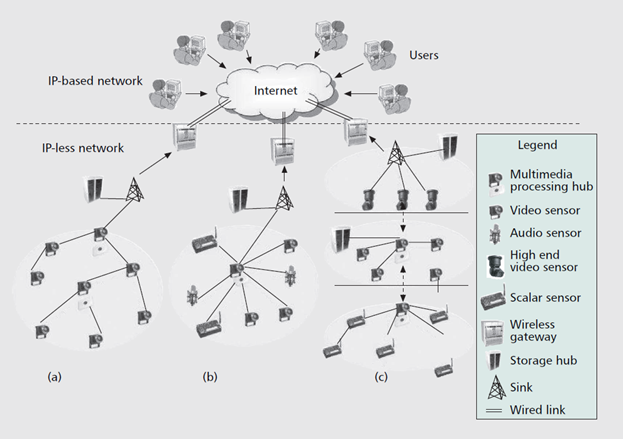
\includegraphics[width=8cm, height=6cm]{images/p1.png}
    \centering
    \caption{Figure 1. Arhitecture of a Wireless Multimedia Sensor Network from} \citet{Hamd01}
\end{figure}

The reference architecture of a wireless multimedia sensor network: (from \citet{Inaf02}
\\ \indent a) single-tier flat, homogeneous sensors, distributed processing, centralized storage; 
\\ \indent b) single-tier clustered, heterogeneous sensors, centralized processing, centralized storage; 
\\ \indent c) multitier, heterogeneous sensors, distributed processing, distributed storage.
\\ \indent The users connect through the Internet and issue queries to a deployed sensor network. The functionality of the various network components are enumerated in the following list:
\\ \indent \textbf{Standard Video and Audio Sensors}. These sensors capture sound or moving images of the sensed event and are typically of low resolution (in terms of pixel/inch for the video sensors and in dB for the audio sensors). They can be arranged in a single-tier network, as shown in the first cloud from the Figure 1, or in a hierarchical manner, as shown in the third cloud.
\\ \indent \textbf{Scalar Sensors}. These sensors sense scalar data and physical attributes, such as temperature, pressure, and humidity and report measured values to their clusterhead. They are typically resource-constrained devices in terms of energy supply, storage capacity, and processing capability.
\\ \indent \textbf{Storage Hubs}. Depending upon the application, the multimedia stream is desired in real time or after further processing. These storage hubs allow data-mining and feature-extraction algorithms to identify the important characteristics of the event, even before the data is sent to the end user.
\\ \indent \textbf{Sink}. All nodes can perform any function such as image capturing, multimedia processing and data transferring to sink over a multi-hop path. The sink is responsible for packaging high level user queries to network specific directives and returning filtered portions of the multimedia stream back to the user. Multiple sinks may be required in a large or heterogeneous network.
\\ \indent \textbf{Gateway}. This serves as the last mile connectivity by bridging the sink to the Internet and is also the only IP-addressable component of the WMSN. It maintains a geographical estimate of the area covered under its sensing framework to allocate tasks to the appropriate sinks that forward sensed data through it.
\\ \indent \textbf{Users}. Users are the highest end of the hierarchy and issue monitoring tasks to the WMSN based on geographical regions of interest. They are typically identified through their IP addresses and run application-level software that assigns queries and displays results obtained from the WMSN.
\\ \indent All of these components are required to form a Wireless Multimedia Sensor Network, the most important components being the sensors which create the network itself, the gateway used to send the information further and lastly the users that benefit from the applications which will be explained in the next chapter. The architectures used are of several types, based on their components order and connections.
\\ \indent Firstly, we will talk about the Single-tier flat architecture, In this architecture the network consists of homogeneous sensor nodes with same capabilities and functionalities. All nodes can perform any function such as image capturing, multimedia processing and data transferring to sink over a multi-hop path, as shown in the next figure:

\begin{figure}
    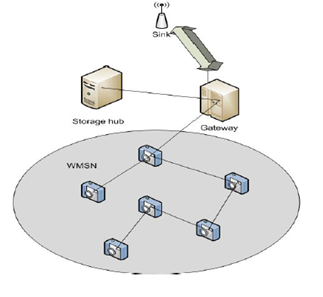
\includegraphics[width=8cm, height=6cm]{images/p2.png}
    \centering
    \caption{Figure 2. Single-tier flat architecture (from \citet{Inaf02}}
\end{figure}

\par \indent The second type is named Single-tier clustered architecture, this type of architecture consists of heterogeneous sensors such as camera, audio and scalar sensors grouped together to form a cluster. All heterogeneous sensors belonging to the same cluster send their sensed data to the cluster head which has more resources and can perform complex data processing. The cluster head is connected either directly or indirectly to the sink or the gateway through multihop path.

\begin{figure}
    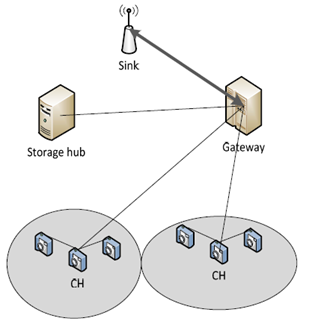
\includegraphics[width=8cm, height=6cm]{images/p3.png}
    \centering
    \caption{Figure 3. Single-tier clustered architecture (from \citet{Inaf02}}
\end{figure}

\par \indent The third is Multi-tier architecture. For this architecture, the first tier consists of scalar sensors that perform simple tasks, like measuring scalar data from surrounding environment (e.g., light, temperature..etc), the second tier consists of camera sensors that perform more complex tasks such as image capturing or object recognition, and at the third tier consists of more powerful and high resolution video camera sensors that are capable of performing more complex tasks, like video streaming or object tracking. Each tier has a central hub for data processing and communicating with the upper tier. The third tier is connected with the sink or the gateway through a multi-hub path.

\begin{figure}
    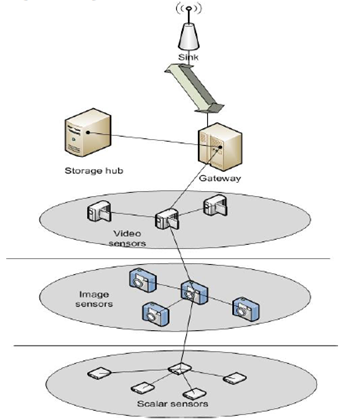
\includegraphics[width=8cm, height=6cm]{images/p4.png}
    \centering
    \caption{Figure 4. Multi-tier architecture (from \citet{Inaf02}}
\end{figure}


\section{Applications of Wireless Multimedia Sensor Networks}

\par \indent These types of networks have the potential and ability to enable many new applications, here are a few examples:
\par \indent \textbf{Multimedia Surveillance Sensor Networks}. Surveillance sensor networks will be used to enhance and complement existing surveillance systems to prevent crime and terrorist attacks. Multimedia content, such as video streams and still images, as well as computer vision techniques, can be used to locate missing persons, identify criminals or terrorists, or infer and record other potentially relevant activities (thefts, car accidents, traffic violations). (from \citet{Inaf02}
\par \indent \textbf{Smart Homes}. Smart homes applications used to automate the life of residences. They are usually used to adapt the house environment according to the residence preferences (e.g., lighting or air conditioning, heating) based on detecting the presence of certain persons inside the house.  (from \citet{Mar04})
\\ \indent \textbf{Traffic Avoidance, Enforcement, and Control Systems}. It will be possible to monitor car traffic in big cities or on highways and deploy services that offer traffic routing advice to avoid congestion or identify violations. In addition, smartparking advice systems based on WMSNs will detect available parking spaces and provide drivers with automated parking advice. (from \citet{Hamd01})
\\ \indent \textbf{Advanced Health Care Delivery}. Telemedicine sensor networks can be integrated with third and fourth generation (3G/4G) cellular networks to provide ubiquitous health care services. Patients will carry medical sensors to monitor parameters such as body temperature, blood pressure, pulse oximetry, ECG, and breathing activity. Remote medical centers will monitor the condition of their patients to infer emergency situations. (from \citet{Hamd01})
\\ \indent \textbf{Environmental and Structural Monitoring}. Arrays of video sensors already are used by oceanographers to determine the evolution of sandbars using image processing techniques. Video and imaging sensors also are used to monitor the structural health of bridges or other civil structures. (from \citet{Hamd01})
\\ \indent \textbf{Industrial Process Control}. Multimedia content such as imaging, temperature, or pressure, can be used for time-critical, industrial, process control. In automated manufacturing processes, the integration of machine vision systems with WMSNs can simplify and add flexibility to systems for visual inspections and automated actions. \citet{Inaf02}
\\ \indent \textbf{Environmental monitoring}. Environmental monitoring application used for monitoring remote and unreachable areas over a long period of time. In these applications, energy-efficient operations are particularly important in order to extend monitoring over a long period of time. (from \citet{Mar04})

\section{Conclusion} 
\label{sec:conclusion}

\par \indent In this paper, were introduced WMSNs technologies and their different applications along with the types of networks they can be constructed as. The main architecture and it’s components were shown and discussed along with examples and day to day usage of the Wireless Multimedia Sensor Networks. It is believed that this research area will attract the attention of many researchers and that it will push one step further our ability to observe the physical environment and interact with it. 


\bibliographystyle{plainnat}
\bibliography{references}

\end{document}


